\documentclass[norsk,a4paper,12pt]{article}
\usepackage[utf8]{inputenc}
\usepackage[T1]{fontenc} %for å bruke æøå
\usepackage[utf8]{inputenc}
\usepackage{graphicx} %for å inkludere grafikk
\usepackage{verbatim} %for å inkludere filer med tegn LaTeX ikke liker
\usepackage{mathpazo}
\usepackage{amsmath}
\usepackage{float}
\usepackage{amsmath}
\usepackage{hyperref}
\newcommand\numberthis{\addtocounter{equation}{1}\tag{\theequation}}
\bibliographystyle{plain}

\begin{document}
\title{Using the Jacobi algorithm for solving eigenvalue problems}
\author{Marcus Berget, Sebastian Amundsen, Andreas Wetzel}
\date{August 2020}
\maketitle

\begin{abstract}
The aim of this project is solving eigenvalue/eigenvector problems using the Jacobi algorithm. Specifically, we will look at solving the Schroedinger's equation with a three-dimensional harmonic oscillator potential. We were able to develop a code which solves the eigenvalue problem for the buckling beam problem with an accuracy of 1e-14, but only an accuracy of 0.1 for the quantum case. When solving eigenvalue problems with the Jacobi method, the number of iterations needed increases quadratic with the dimension of the matrix used. In other words, there is a trade-off between precision and time which needs to be taken into account when solving eigenvalue problems with the Jacobi algorithm. 
\end{abstract}

\section{Introduction}

The aim of this project is solving eigenvalue/eigenvector problems using the Jacobi algorithm. Specifically, we will look at solving the Schroedinger's equation with a three-dimensional harmonic oscillator potential. 

\section{Theory}

We will look at the two point boundary problem of a buckling beam. This problem has analytical solutions, which can be used to check the accuracy of a numerical approximation. The differential equation we wish to solve for the beam of length L is:

\begin{equation}
\gamma \frac{d^2 u(x)}{dx^2}=-Fu(x)  \hspace{1cm}  x \in [0,L]
 \label{eq:de}
 \end{equation}

Where u(x) is the displacement of the beam in the y direction, F is the force applied at (L,0) and $\gamma$ is a constant. We apply the Dirichlet boundary conditions and set u(0)=u(L)=0. Two of the parameters are known, say F and L. We then set up an eigenvalue problem to find $\gamma$. We can rewrite equation \ref{eq:de} as:

\begin{equation}
\gamma \frac{d^2 u(\rho)}{dx^2}=-\frac{FL^2}{\gamma}u(\rho)=-\lambda u(\rho)  \hspace{1cm}  \rho \in [0,1]
 \label{eq:de2}
 \end{equation}

With $\lambda=FL^2/\gamma$, the equation can be solved as an eigenvalue problem.

The first step of solving eigenvalue problems numerically, is of course to set up the matrix. In both the case of solving the buckling beam problem and the quantum mechanical problem the matrix is a tridiagonal matrix. This matrix is given by rewriting the expression for the second derivative of a function u:

$$
u'' = \frac{u(p+h)-2u(p) + u(p-h)}{h^2} + O(h^2)
$$

Where $h=\frac{\rho_N-\rho}{N}$ is our step length, $\rho_N=1$ and $\rho_0=0$. This expression can be rewritten as:

$$
-\frac{u_{i+1}-2u_i+u_{i-1}}{h^2}=\lambda u_i
$$

We can rewrite this equation as an eigenvalue problem:

\begin{equation}
    \begin{bmatrix} d& a & 0   & 0    & \dots  &0     & 0 \\
                                a & d & a & 0    & \dots  &0     &0 \\
                                0   & a & d & a  &0       &\dots & 0\\
                                \dots  & \dots & \dots & \dots  &\dots      &\dots & \dots\\
                                0   & \dots & \dots & \dots  &a  &d & a\\
                                0   & \dots & \dots & \dots  &\dots       &a & d\end{bmatrix} 
                                 \begin{bmatrix} u_1 \\ u_2 \\ u_3 \\ \dots \\ u_{N-2} \\ u_{N-1}\end{bmatrix} = \lambda \begin{bmatrix} u_1 \\ u_2 \\ u_3 \\ \dots \\ u_{N-2} \\ u_{N-1}\end{bmatrix} . 
\label{eq:matrix} 
\end{equation}

The diagonal elements are defined as $d=2/h^2$ and the non-diagonal elements are defined as $a=-1/h^2$. This eigenvalue problem has analytical eigenpairs, with corresponding eigenvalues:
\[
\lambda_j = d+2a\cos{(\frac{j\pi}{N})}, \hspace{1cm} j=1,2,\dots N-1.
\]

The associated eigenvectors are:
\[
\mathbf{u}_j = [ \sin(\frac{j\pi}{N}), \sin(\frac{2j\pi}{N}), ..., \sin(\frac{(N-1)j\pi}{N}) ]^T, \hspace{0.2cm} j=1,2,\dots N-1.
\]

We define $\tan\theta = t= s/c$, where $s=\sin\theta$ and $c=\cos\theta$. We also have:
\begin{equation*}\cot 2\theta=\tau = \frac{a_{ll}-a_{kk}}{2a_{kl}}.
\end{equation*}

We obtain the quadratic equation:

\begin{equation*}
t^2+2\tau t-1= 0,
\end{equation*}
 which we use to find t:
 
\begin{equation*}
  t = -\tau \pm \sqrt{1+\tau^2},
\end{equation*}
which gives us the variables c and s:

\begin{equation*}
   c = \frac{1}{\sqrt{1+t^2}},
   \label{eq:c} 
\end{equation*}

\begin{equation*}
  s=ct
   \label{eq:s} 
\end{equation*}


The general expression for the new matrix elements are:
$$
b_{ii}=a_{ii}, i\neq k, i\neq l \\
$$
$$
b_{ik}=a_{ik}\cos \theta - a_{il}\sin \theta, i\neq k, i\neq l
$$
$$
b_{il}=a_{il}\cos\theta+a_{ik}\sin\theta, i\neq k, i\neq l
$$
$$
b_{kk}=a_{kk} \cos^2\theta - 2a_{kl}\cos\theta \sin\theta + a_{ll}\sin^2\theta
$$
$$
b_{ll}=a_{ll}\cos^2\theta+2a_{kl}\cos\theta \sin\theta + a_{kk}\sin^2\theta
$$
\begin{equation}
b_{kl} = (a_{kk}-a_{ll})\cos\theta\sin\theta+a_{kl}(\cos^2\theta-\sin^2\theta)
 \label{eq:Jacob}
 \end{equation}

Where we insert the expressions for c and s.

We will study two electrons in a harmonic oscillator well. The radial Schrödinger equation in this case is:

\begin{equation*}
\left(  -\frac{\hbar^2}{m} \frac{d^2}{dr^2} -\frac{\hbar^2}{4 m} \frac{d^2}{dR^2}+ \frac{1}{4} k r^2+  kR^2\right)u(r,R)  = E^{(2)} u(r,R).
\end{equation*}

Were we have introduced the relative coordinate $\mathbf{r} = \mathbf{r}_1-\mathbf{r}_2$
and the center-of-mass coordinate $\mathbf{R}=1/2(\mathbf{r}_1+\mathbf{r}_2)$. With some manipulation and calculation we arrive at a form which can be solved using the Jacobi method (for calculations and definitions see \cite{94}):

\begin{equation}
  -\frac{d^2}{d\rho^2} \psi(\rho) + \omega_r^2\rho^2\psi(\rho) +\frac{1}{\rho} = \lambda \psi(\rho).
\label{eq:SE}
\end{equation}

Where $\omega_r$ is a parameter which reflects the strength of the oscillator potential.

\section{Method}
All the code can be found at: \\
\url{https://github.com/Sebamun/FYS3150_Projekter/tree/master/Prosjekt2/Prosjekt2_kode}
\\


In the case of the buckling beam problem the matrix becomes very simple, the diagonal elements are all equal (d in equation \ref{eq:matrix}), and the non-diagonal elements are all equal (a in equation \ref{eq:matrix}). 

We wish to solve equation \ref{eq:matrix} by using Jacobi's rotation algorithm. First we find the variables c and s from equation \ref{eq:c} and equation \ref{eq:s}. These values are to be implemented in the expression for the new matrix elements given equation \ref{eq:Jacob}.

We wish to find out how many similarity transformations we need before all the non-diagonal elements are essentially zero. We wish to illustrate this by plotting the number of Jacobi rotations needed against the dimension of the matrix. 

We are also going to compare the eigenvector with the lowest eigenvalue with the analytical solution. We find the analytical eigenvalues by using armadillos functions for diagonalizing a matrix. These values are to be compared with values found using the Jacobi method. 


We will solve equation \ref{eq:SE} using the values $\omega_r = 0.01$, $\omega_r = 0.5$, $\omega_r =1$ and $\omega_r = 5$ for the ground state. We will use the same method as we did for the buckling beam. The only difference being that we add the potential $\omega_r^2\rho^2+1/\rho$ to the diagonal elements.

\section{Implementation}

\section{Results}
\begin{figure}[H]
	\centering
	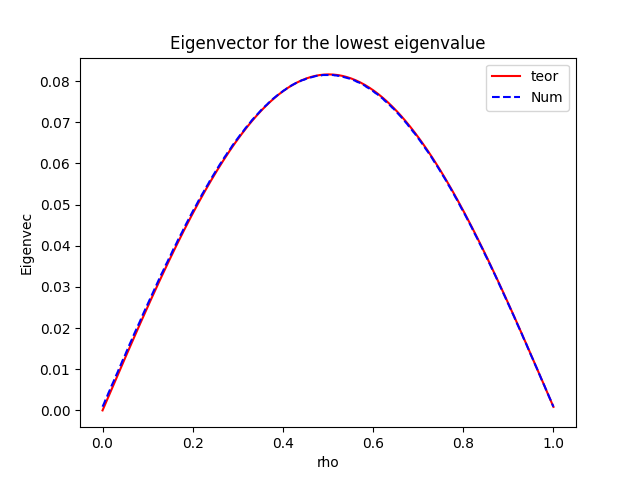
\includegraphics[width=\linewidth]{Egenvektorer1.png}
	\caption{Above we see a plot of the eigenvector for computed with the armadillo function $\text{eig\_sym}$ ($\text{Num}$), vs. the theoretical eigenvector (teor). This is for the buckling beam problem.}
	\label{fig:egen1}
\end{figure}

\begin{figure}[H]
	\centering
	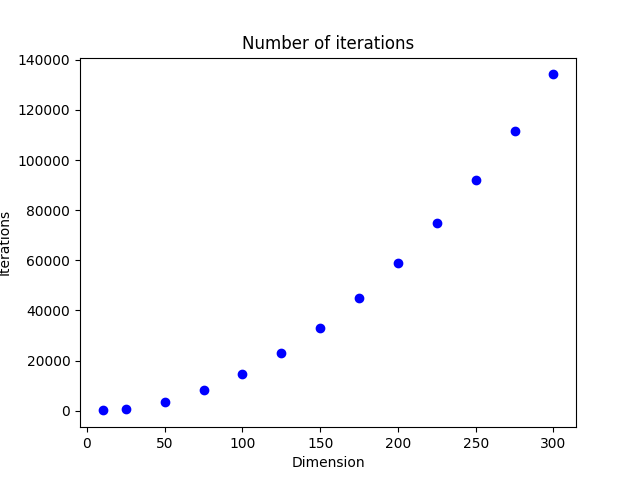
\includegraphics[width=\linewidth]{Iterasjoner.png}
	\caption{Above we have plotted the number of Jacobi rotations needed to make the non-diagonal elements essentially zero against the dimension of the matrix. (Buckling beam)}
	\label{fig:iter}
\end{figure}

\begin{figure}[H]
	\centering
	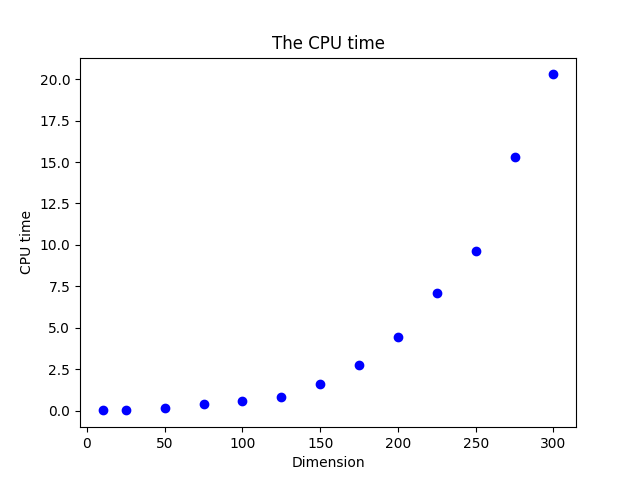
\includegraphics[width=\linewidth]{CPU_tid.png}
	\caption{Above we have plotted the CPU-time needed to make the non-diagonal elements essentially zero against the dimension of the matrix. (buckling beam)}
	\label{fig:CPU}
\end{figure}

For the buckling beam eigenvalue problem we were able to reproduce the eigenvalues with an accuracy of 1e-14 compared to the analytical values. For the case with quantum dots in three dimensions and one electron, we tried to find how many integration points was needed to reproduce the analytical results with four leading digits after the decimal point. For some reason, we weren't able to reproduce the analytical results with more than one leading digit after the decimal point. 

\begin{figure}[H]
	\centering
	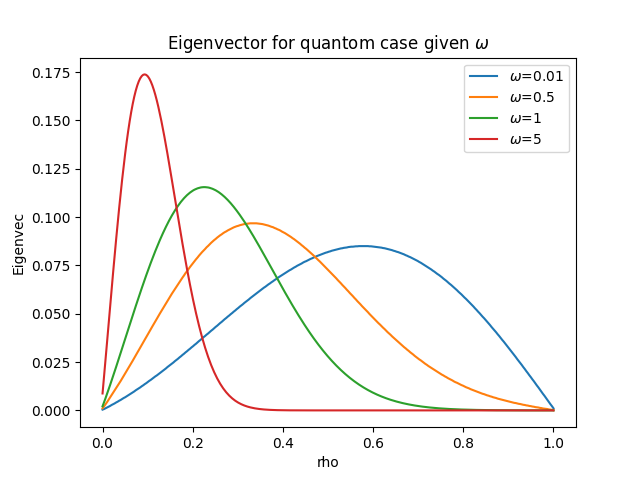
\includegraphics[width=\linewidth]{Egenvektorer_omega.png}
	\caption{Above we have plotted the eigenvectors for the quantum case with different values for $\omega$}
	\label{fig:omega}
\end{figure}

\section{Discussion}
From Figure (\ref{fig:egen1}) we can see that armadillo's function for computing eigenvectors seem to be very accurate which gives a good comparison tool when checking whether our code works. When looking at Figure (\ref{fig:iter}), it seems that the number of iterations against the dimension increases in a quadratic fashion. This might make sense, given the fact that the elements of a matrix also increases quadratic with the dimension. When looking at Figure (\ref{fig:CPU}), we can see that the CPU-time needed, seems to increase at an even faster rate. This might be due to the fact that at higher dimensions, the RAM might max out making the time needed per iteration higher for higher dimensions. As stated above, we weren't able to reproduce the analytical eigenvalues for the quantum case with one electron with more than one leading digit after the decimal point. We couldn't find the reason for why we couldn't, even though we tried different values for $\rho_{max}$ between 1 and 10, increasing the dimension, and adjusting the tolerance for the Jacobi algorithm. In addition, due to poor workflow management and a quite chaotic code we lost the data for the eigenvalues in both the buckling beam problem and the quantum case. We could've tried to reproduce them, but at this point we simply don't have the time for that. We believe that better planning and by using object oriented code, we could've avoided this specific problem. Finally, looking at Figure (\ref{fig:omega}) we see the eigenvectors for the quantum case using different values for $\omega$. Unfortunately we couldn't access the analytical solutions for the eigenvectors (due to every group member being in quarantine), so we are unable to tell if the eigenvectors we found represent the correct solutions. Furthermore, we would like to comment on the overall unrefined touch of the report/code. The unexpected sickness in addition to group members being infected with the COVID-19 disease caught us by surprise and we were not ready for it. Though we are not using these events as an excuse, we have learned that with better workflow planning, communication and organizing we would've been more prepared for it. This is definitely an experience we will bring with us to future projects.  

\section{Concluding remarks}

We were able to develop a code which solves the eigenvalue problem for the buckling beam problem with great accuracy, but encountered problems achieving the same accuracy for the quantum case. When solving eigenvalue problems with the Jacobi method, the number of iterations needed increases quadratic with the dimension of the matrix used. In other words, there is a trade-off between precision and time which needs to be taken into account when solving eigenvalue problems with the Jacobi algorithm. 

\begin{thebibliography}{9}
\bibitem{94}
	Department of Physics, University of Oslo, Norway, 2020 Project 2 (Computational Physics I FYS3150/FYS4150)
\end{thebibliography}


\end{document}
